%%%%%%%%%%%%%%%%%%%%%%%%%%%%%%%%%%%%%%%%%%%%%%%%%%%%%%%%%%%%%%%%%%%%%%%%%%%%%%%%%%
\begin{frame}[fragile]\frametitle{}
\begin{center}
{\Large Implementation}
\end{center}
\end{frame}


%%%%%%%%%%%%%%%%%%%%%%%%%%%%%%%%%%%%%%%%%%%%%%%%%%%%%%%%%%%
\begin{frame}[fragile]\frametitle{How to build GraphRAG?}

	\begin{center}
	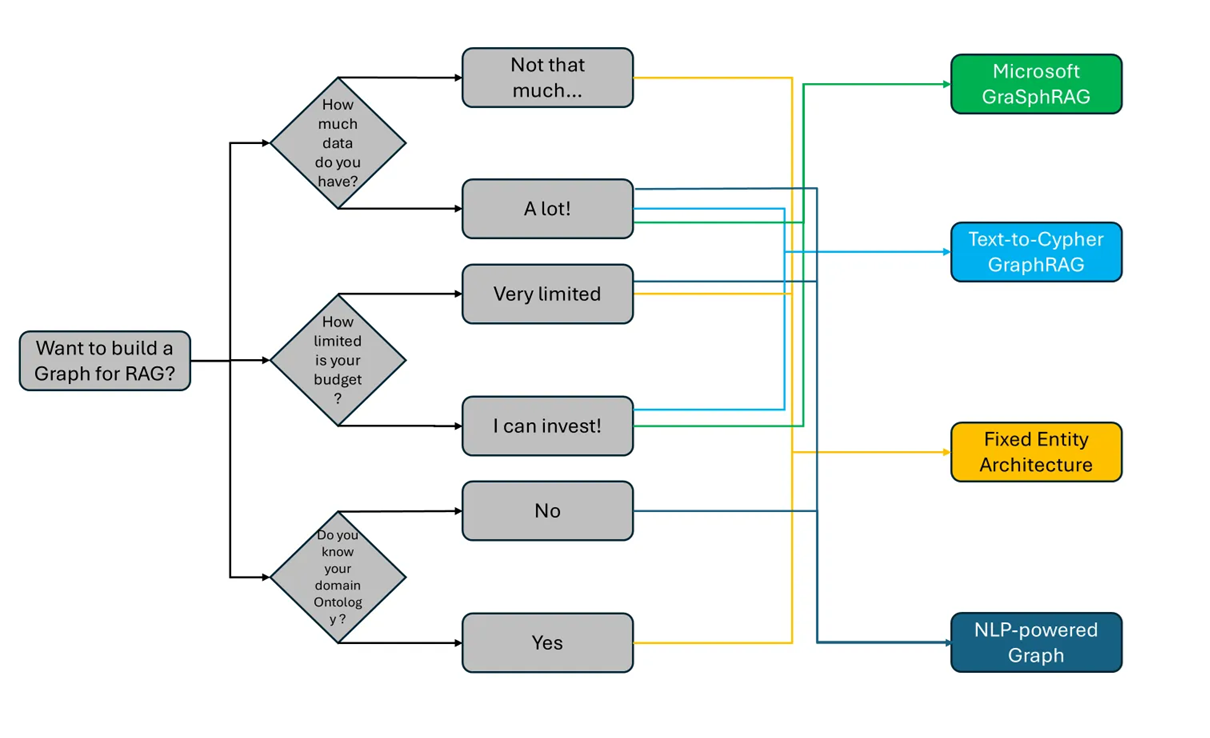
\includegraphics[width=\linewidth,keepaspectratio]{graphrag1}
	
	{\tiny (Ref: Build your hybrid-Graph for RAG \& GraphRAG applications using the power of NL - Irina Adamchic)}
	\end{center}
	
\end{frame}


%%%%%%%%%%%%%%%%%%%%%%%%%%%%%%%%%%%%%%%%%%%%%%%%%%%%%%%%%%%
\begin{frame}[fragile]\frametitle{Neo4j Ollama GraphRAG}

	\begin{center}
	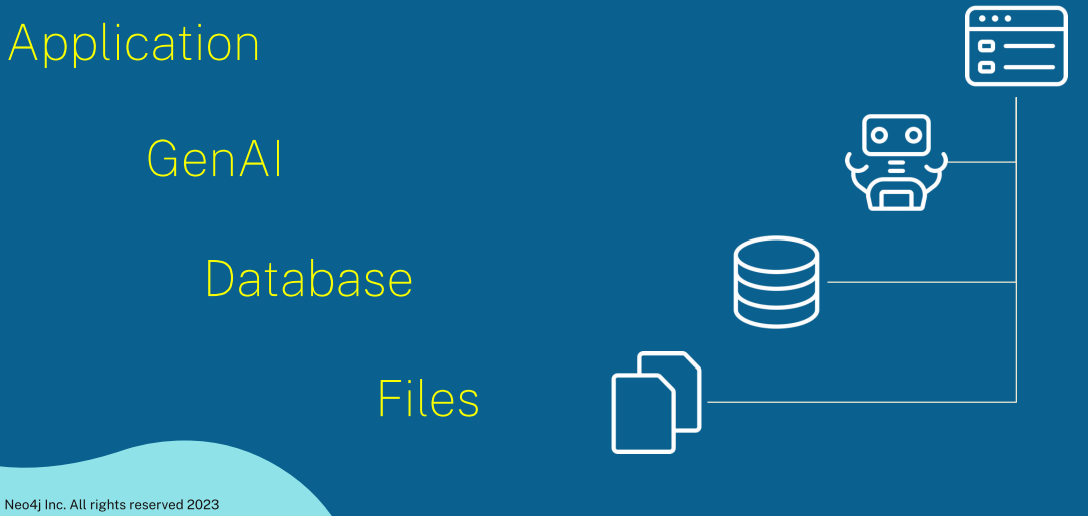
\includegraphics[width=0.6\linewidth,keepaspectratio]{graphrag2}
	
	{\tiny (Ref: The GenAI Stack - Andreas Kollegger - Neo4j)}
	\end{center}
	
	    \begin{itemize}
        \item Application: LangChain: an ``orchestration framework'' for integrating with LLMs
		\item Gen AI : Ollama : locally managed language models
		\item Database: Neo4j: knowledge graph to augment the LLM
		\item Files: import: sample data sources for constructing a knowledge graph
    \end{itemize}
\end{frame}

